% !TeX TXS-program:compile = txs:///pdflatex/[--shell-escape]
\documentclass[handout, aspectratio=169, 10pt]{beamer}

% packages
\usepackage{newpxmath} % math font is Palatino compatible
% \usepackage[nomath]{fontspec}

\usepackage{setspace}
\usepackage{xcolor}
\usepackage{soul} % for \st
\usepackage{hyperref} % for links
\definecolor{links}{HTML}{2A1B81}
\hypersetup{colorlinks,linkcolor=,urlcolor=links}


% table stuff
\usepackage{chronosys}
\usepackage{verbatim}
% \pagenumbering{arabic}
\usepackage{tabularx}
\usepackage{booktabs}
\usepackage{ragged2e}
\usepackage{mathtools}

% R Code
\usepackage{listings}
\usepackage{courier}
\lstset{basicstyle=\scriptsize\ttfamily,breaklines=true}
\lstset{framextopmargin=50pt,frame=bottomline}

% themes
\usetheme[progressbar=frametitle, block=fill]{metropolis}
\useoutertheme{metropolis}
\useinnertheme{metropolis}

% colors
\definecolor{dimwhite}{rgb}{0.99, 0.99, 0.99}
\definecolor{charcoal}{rgb}{0.21, 0.27, 0.31}
\definecolor{slategray}{rgb}{0.44, 0.5, 0.56}
\definecolor{dimgray}{rgb}{0.41, 0.41, 0.41}
\definecolor{bleudefrance}{rgb}{0.19, 0.55, 0.91}

% beamer options
\setbeamercolor{author}{fg=charcoal}
\setbeamercolor{background canvas}{bg=white}
\setbeamercolor{section in toc}{fg=charcoal}
\setbeamercolor{subsection in toc}{fg=dimgray}
\setbeamercolor{frametitle}{bg=dimwhite, fg=charcoal}
\setbeamercolor{progress bar}{fg=slategray, bg=fg!50!black!30}
\setbeamercovered{transparent}
\setbeamertemplate{itemize items}[triangle]
\setbeamertemplate{itemize subitem}[circle]
\setbeamertemplate{itemize subsubitem}[square]
\setbeamersize{text margin left=7mm,text margin right=7mm} 

% new commands
\newcommand{\q}[1]{``#1''}
\newcommand{\hs}[1]{\textsc{\hfill\scriptsize\color{dimgray}#1}}
\newcommand{\g}[1]{{\color{gray}#1}}
\newcommand{\dg}[1]{{\color{dimgray}#1}}
\newcommand{\sg}[1]{{\color{slategray}#1}}
\newcommand{\bdf}[1]{{\color{bleudefrance}#1}}
\newcommand{\itemcolor}[1]{\renewcommand{\makelabel}[1]{\color{#1}\hfil ##1}}
\newcommand\Wider[2][2em]{
\makebox[\linewidth][c]{
  \begin{minipage}{\dimexpr\textwidth+#1\relax}
  \raggedright#2
  \end{minipage}
  }
}

% misc
\linespread{1.35}

% minted (risky)
\usepackage[cache=false]{minted}

% Math stuff
\newcommand{\norm}[1]{\left\lVert#1\right\rVert}
\newcommand{\R}{\mathbb{R}}
\newcommand{\E}{\mathbb{E}}
\newcommand{\V}{\mathbb{V}}
\newcommand{\probP}{\text{I\kern-0.15em P}}
\newcommand{\ol}{\overline}
%\newcommand{\ul}{\underline}
\newcommand{\pp}{{\prime \prime}}
\newcommand{\ppp}{{\prime \prime \prime}}
\newcommand{\policy}{\gamma}
\newcommand{\plim}{ \overset{p}{\to}}
\newcommand{\hnot}{ \overset{H_0}{\to}}

% Causal Graphs
\usetikzlibrary{shapes,decorations,arrows,calc,arrows.meta,fit,positioning}
\tikzset{
    -Latex,auto,node distance =1 cm and 1 cm,semithick,
    state/.style ={ellipse, draw, minimum width = 0.7 cm},
    point/.style = {circle, draw, inner sep=0.04cm,fill,node contents={}},
    bidirected/.style={Latex-Latex,dashed},
    el/.style = {inner sep=2pt, align=left, sloped}
}

\setbeamersize{text margin left=10pt,text margin right=10pt}


\begin{document}


\title[L5-Wage Equation Example]{ Econometrics I}
\subtitle{Lecture 5: Extended Example: The Wage Equation}
\author{Chris Conlon}
\date{Fall 2025}
\maketitle






\begin{frame}{Mincerian Regression}
\begin{itemize}
	\item Recall the Mincerian regression (wage equation):\[
	\ln wage_i = \beta_0 + \beta_{ed} Education_i + \beta_{exp} Experience_i + \beta_{Fem} Female_i + \dots + \varepsilon_i
	\]

	\smallskip
	\item Let's revisit estimating this with the Cornwell and Rupert (NLSY) data. 
\end{itemize}
\end{frame}




\begin{frame}{Process the data}
\begin{center}
	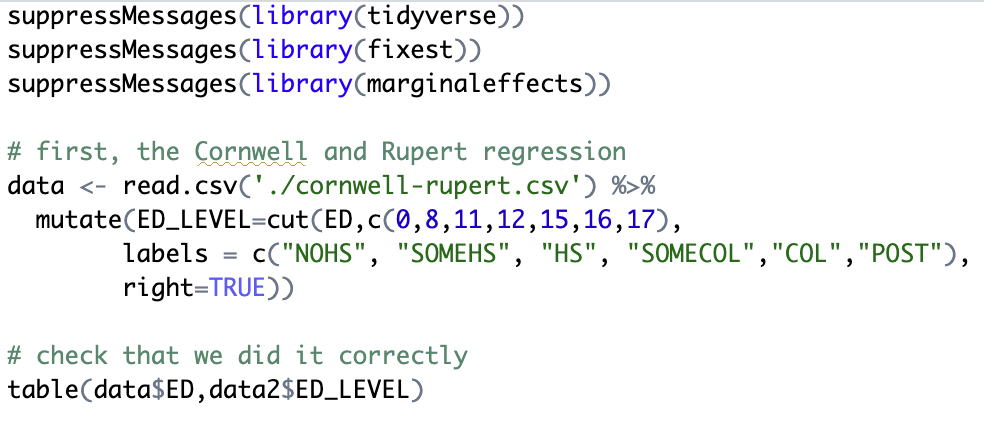
\includegraphics [width=.9\textwidth]{code_0}\\
\end{center}
\end{frame}



\begin{frame}{Baseline Results}
\begin{columns}
\begin{column}{0.6\textwidth}
\begin{figure}
\flushleft
	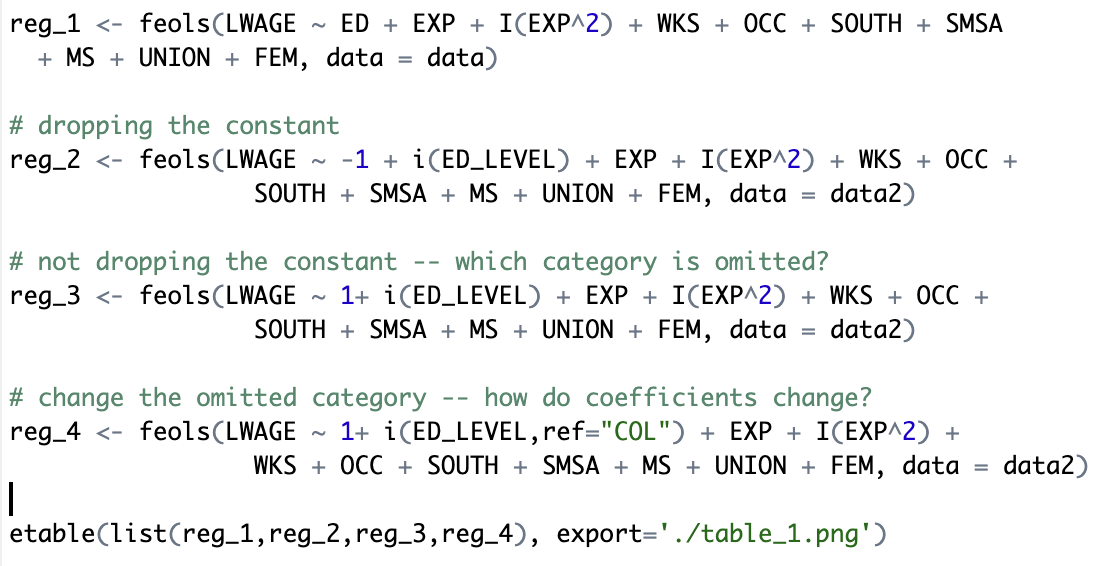
\includegraphics [width=\textwidth]	{code_1}
\end{figure}
Note on interpreting effects with log dependent variable:

Intrepreting coefficients for $\log(y_i)\approx 1+\beta$:
\begin{itemize}
	\item $\exp \left( -.3892\right) = .6826$
		\item $\exp \left( .05654\right) = 1.057$
\end{itemize}

\end{column}
\begin{column}{0.4\textwidth}
\begin{figure}
\flushleft
	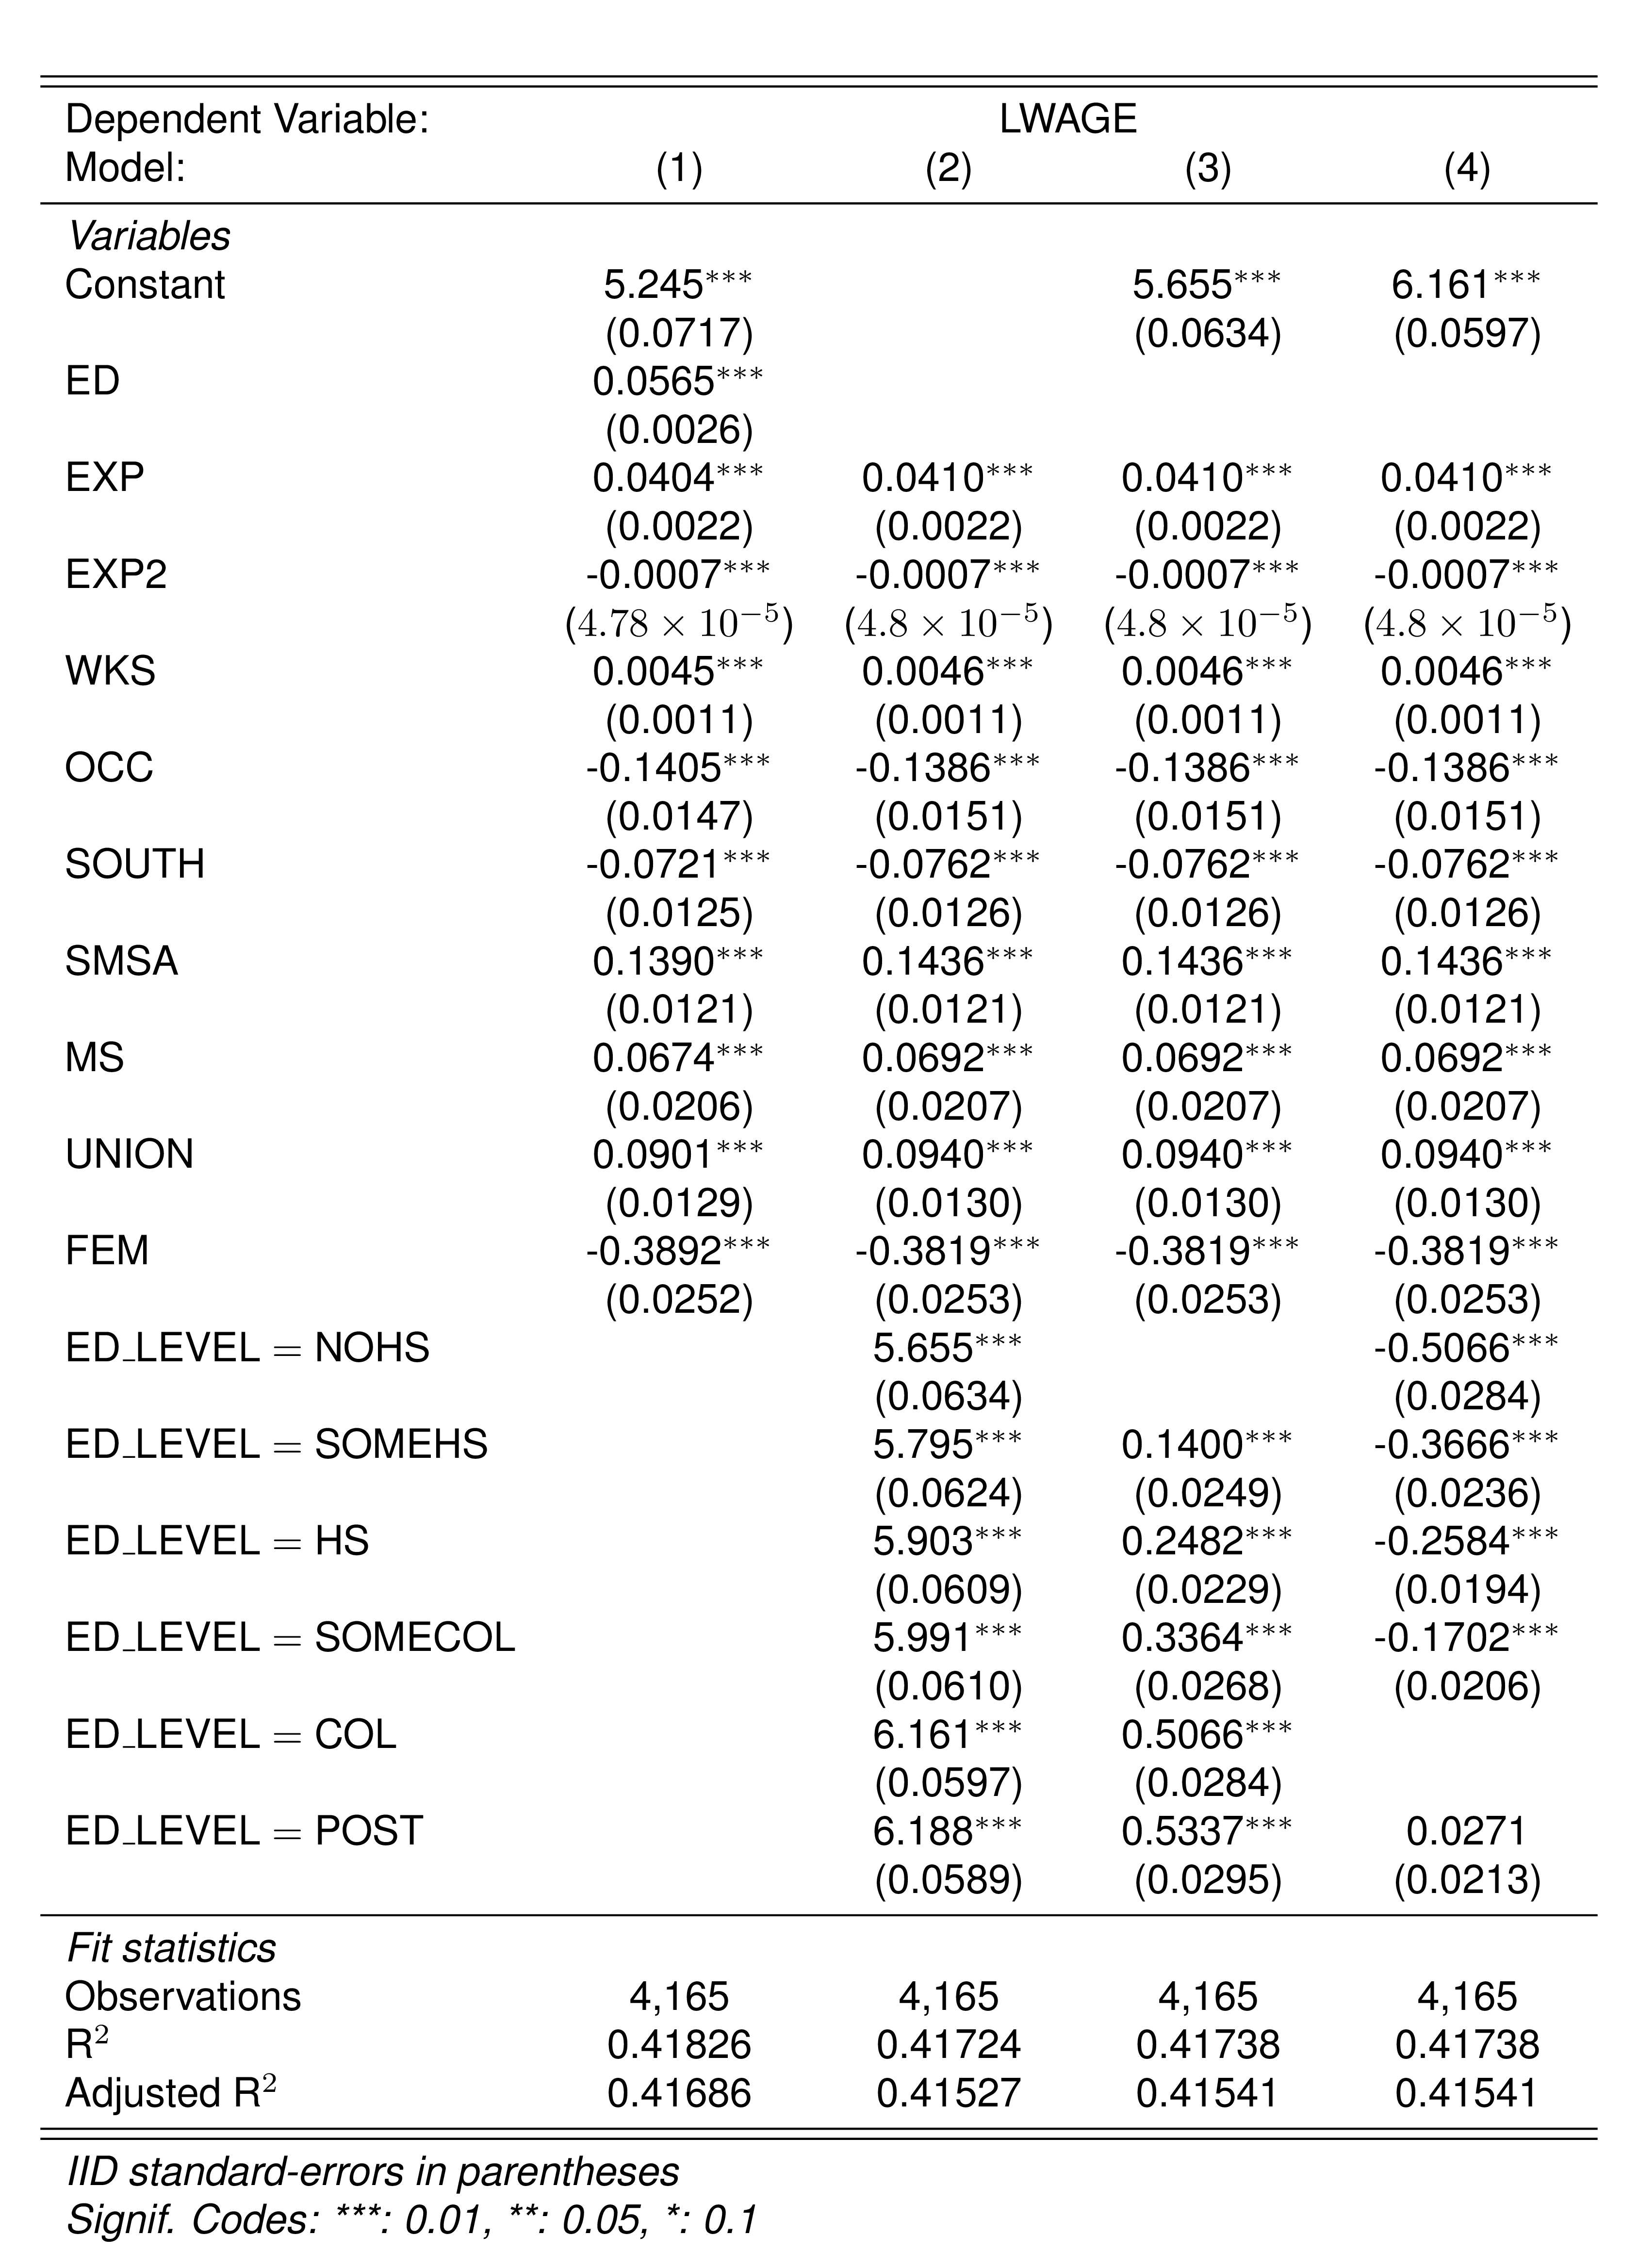
\includegraphics [width=\textwidth]	{table_1}
\end{figure}
\end{column}
\end{columns}	

\end{frame}


\begin{frame}[t]
\frametitle{Heuristic Policies}

\begin{columns}

\column{0.5\textwidth}
\begin{itemize}
\item<1-> These are methods aiming to give a good but not necessarily optimal solution to a problem.
\item<2-> There exist a number of such policies for bandit problems.
\alt<1-9>{
\item<3-9> Greedy policy:
\begin{itemize}
\normalsize
\item<4-9> choose arm with greatest expected reward
\item<5-9> ignores variability in prior distribution
\item<6-9> quite good for Bernoulli bandits, but less effective for normal bandits
\end{itemize}
}{\only<10-14>{\item<10-> Next policy:
\begin{itemize}
\normalsize
\item<11-14> comment 1
\item<12-14> comment 2
\item<13-14> comment 3\par
\rule{0pt}{2.7cm}
\end{itemize}}
\only<15-18>{\item<15-> Another policy:
\begin{itemize}
\normalsize
\item<16-18> Another comment 1
\item<17-18> Another comment 2
\item<18-18> Another comment 3\par
\rule{0pt}{2.7cm}
\end{itemize}}
}
\end{itemize}

\column{0.3\textwidth}
\vspace{-25pt}
\uncover<7->{\begin{figure}
\begin{center}
\includegraphics[height = 2.7cm, trim=-1cm 0cm 0cm 0cm,clip=true,width=3cm]{example-image-a}
\caption*{$(\alpha,\beta) = (1,1)$}
\end{center}
\end{figure}}
\vspace{-25pt}
\uncover<8->{
\begin{figure}
\begin{center}
\includegraphics[height = 2.7cm, trim=-1cm 0cm 0cm 0cm,clip=true,width=3cm]{example-image-a}
\caption*{$(\alpha,\beta) = (6,5)$}
\end{center}
\end{figure}}

\column{0.2\textwidth} 
\only<9>{$\Rightarrow$ play this arm} 
\only<13-14>{$\Rightarrow$ play this arm with probability $\varepsilon$\vspace{80pt}} 
\only<14>{$\Rightarrow$ play this arm with probability $1-\varepsilon$} 
\end{columns} 
\onslide<10>{\null}
\end{frame}

\end{document}